\appendix
\chapter{Learned sensing matrices and network parameters}
\subsection{Unsupervised small network}

Figure \ref{fig:Phial} shows the graphical representation of the sensing matrix learned during training. Each small square is interpreted as the subsampling matrix for each input dimension.

\begin{figure}[!htb] 
\vspace{1cm}
\centering 
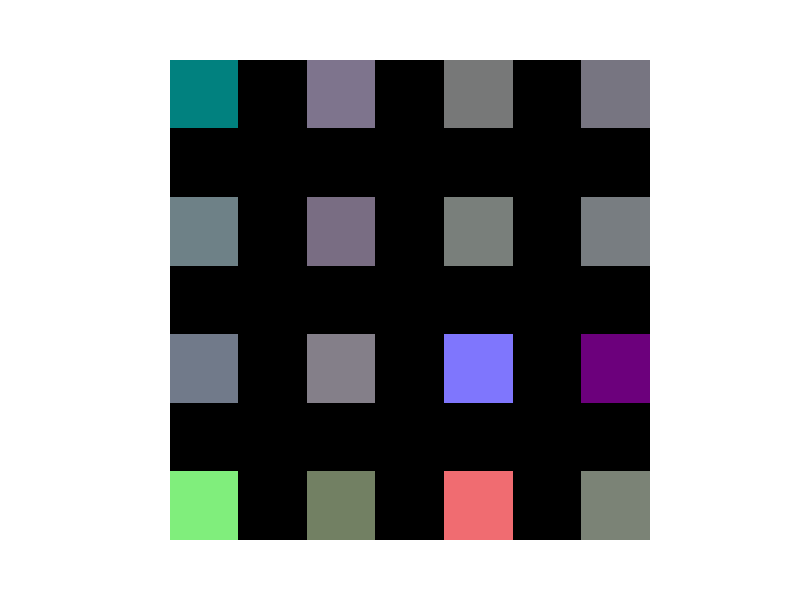
\includegraphics[width=\textwidth,height=\textheight,keepaspectratio=true]{Conv1alpha.png}
\caption[Learned sensing matrix for small network]{Sensing matrix for small network.}
\label{fig:Phial} 
\end{figure} 

\FloatBarrier

%\begin{table}[tb]
%\caption[Details of $\alpha$ Network]{Original features of each dataset.}
%\label{tab:AlphaNetpar}
%\centering
%\begin{tabular}{l*{6}{c}r}
%Number of layers & Size input layer & size output layer & Number of parameters $\omega$%\\
%\hline
%   &  &  &  &  \\
%\bottomrule 
%\end{tabular}  
%\end{table}

\subsection{Unsupervised large network}

Figure \ref{fig:Phial} shows the graphical representation of the sensing matrix learned during training. Each small square is interpreted as the subsampling matrix for each input dimension.

\begin{figure}[!htb] 
\vspace{1cm}
\centering 
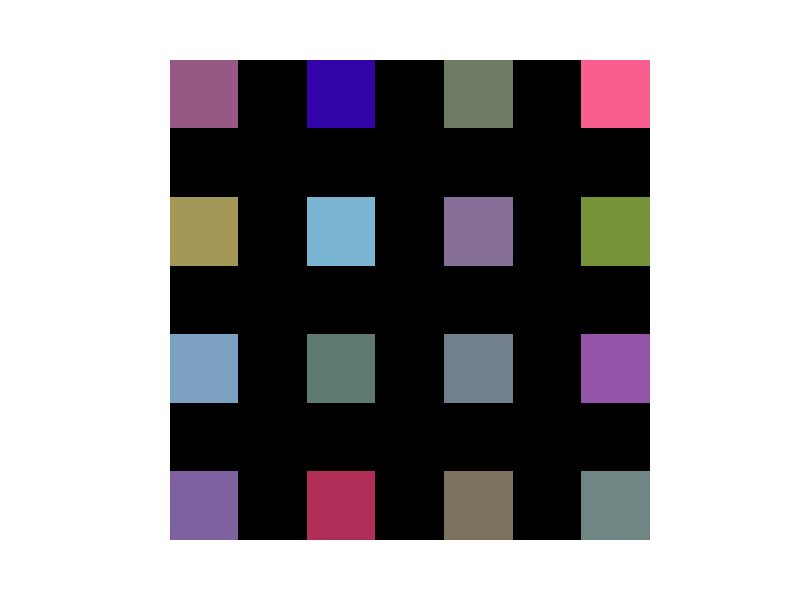
\includegraphics[width=\textwidth,height=\textheight,keepaspectratio=true]{Conv1beta.png}
\caption[Learned sensing matrix for large network]{Sensing matrix for large network.}
\label{fig:Phial} 
\end{figure} 

\FloatBarrier

\subsection{Network implementation settings}

Table \ref{tab:summaryNets} lists the details of each of our networks for reconstruction images.

\begin{table}[!htb]
\caption[Implementation details of each network]{Implementation details of each proposed network.}
\label{tab:summaryNets}
\begin{center}
\resizebox{\textwidth}{!}{
\begin{tabular}{l*{6}{c}r}
Network              & $\#$ of layers & $\#$ hidden layers & $\#$ parameters $\omega$ & appprox. train time\\
\hline
Small Supervised   & 2 & 0 & 313728 &  3.3 hrs\\
Small Unsupervised     & 3 & 1 & 350608 & 4.85 hrs\\
Large Supervised & 3 & 1 & 42766592 & 18 hrs\\
Large Unsupervised & 4 & 2 & 42803472 & 40 hrs\\
\bottomrule 
\end{tabular} }
\end{center}
\end{table}

\FloatBarrier

